`\section{Introduction}

Tool-using language models are increasingly deployed as agents that execute multi-step workflows over external systems: booking, retail operations, and telecom support.
Reliability in this regime means \emph{robustness to tool-context shift}: different tool schemas, argument conventions, and failure modes.

Reinforcement learning (RL) is the cleanest way to optimize end-to-end success from execution feedback.
Yet end-to-end (E2E) RL for tool use has remained largely inaccessible outside well-resourced efforts.
The bottleneck is not the objective; it is iteration cost.
Tool-use episodes are long and sequential, and the standard token-level view of an LLM as an MDP over tokens forces the algorithm to (i) generate long rollouts and (ii) backpropagate advantage through many low-leverage tokens.

\paragraph{Insight 1: the right MDP granularity is the interaction turn.}
Agentic tool use is naturally an episodic decision process where the environment reacts \emph{after} an assistant turn:
the model emits a tool call (tool name + arguments) or a short language act, the tool/environment responds, and only then does the next decision state arise.
This suggests a more appropriate formulation: an \emph{episodic MDP whose actions are turns (structured tool calls / interaction acts), not tokens}.
The resulting \emph{turn-level advantage} is the object that matters for learning which tool/arguments to choose.
This is not a cosmetic change: it reduces the effective horizon from tokens to turns, and it enables reusing cached prefixes as training inputs without repeatedly regenerating entire multi-turn interactions.

\paragraph{Insight 2: advantage is sparse at the turn level.}
Once we adopt the turn-level MDP, a second pattern becomes clear.
Most turns are mechanically determined after the key decisions are made (e.g., formatting, confirmations, and bookkeeping).
At these states, all plausible turns have similar value, so $Q(s,a)\approx V(s)$ and the advantage is near zero.
By contrast, a small number of states dominate success: choosing the right tool, setting critical arguments, or selecting an error-recovery branch.
At those states, one action has much higher value than the baseline, i.e., $Q(s,a)-V(s)$ is large.
We call these \emph{pivot states}.

\paragraph{PivotRL.}
PivotRL combines both ideas:
\begin{itemize}
    \item We optimize the \emph{turn-level} policy gradient, treating each turn as the action and applying advantage at that granularity.
    \item We \emph{concentrate} RL updates on pivot states, updating only the short token span that encodes the structured turn action.
\end{itemize}
This is a compute-allocation principle made concrete: spend RL compute where action choice changes the outcome.

\paragraph{Estimating $Q$ and $V$ without dense branching.}
Turn-level RL still requires estimating which turns are high value at intermediate prefixes.
Dense branching rollouts from many prefixes are expensive.
PivotRL uses a tool-use-specific proxy: generate trajectories from a strong teacher, verify correctness, and treat the teacher turn at shared states as the high-value action.
This yields cheap value comparisons that are particularly appropriate at pivots, where the action-value landscape is close to binary (a narrow set of correct tool calls versus many incorrect ones).

\paragraph{Contributions.}
\begin{itemize}
    \item \textbf{Turn-level MDP formulation for tool-use RL.}
    We formalize agentic tool use as an episodic MDP over interaction turns and derive the corresponding turn-level policy gradient, clarifying the correct advantage granularity for tool calling.
    \item \textbf{Pivot states and sparse advantage at the turn level.}
    We formalize pivots as states with large turn-level advantage gaps and give simple bounds showing why non-pivot states contribute little to the gradient.
    \item \textbf{PivotRL.}
    A turn-level GRPO-style optimization procedure that mines pivots and applies group updates only at pivot turns, reusing cached prefixes and avoiding repeated long-horizon rollouts.
\end{itemize}

\section{Preliminaries: tool use as a turn-level episodic MDP}
\label{sec:mdp}

\paragraph{Tool contexts.}
A \emph{tool context} $c$ specifies available tools (names, signatures, constraints, descriptions) and execution semantics.
A task instance under $c$ induces an episodic interaction between an agent and an environment (tools + user).

\paragraph{Turn-level MDP.}
We model this interaction as an episodic MDP
\[
M_c = (\mathcal{S}_c, \mathcal{A}_c, P_c, r_c, \gamma, \rho_c),
\]
where:
\begin{itemize}
    \item $s\in\mathcal{S}_c$ is an \emph{interaction prefix}: system prompt, user goal, dialogue history, tool outputs, and tool-call metadata.
    \item $a\in\mathcal{A}_c(s)$ is a \emph{turn action}: a complete assistant turn, typically a structured tool call (tool name + arguments) or a short natural-language act (e.g., asking a clarifying question).
    \item The transition $s'\sim P_c(\cdot\mid s,a)$ is induced by executing the tool call (if any) and appending the resulting observation(s) to the transcript.
    \item Rewards are task-level (often sparse): e.g., success at termination.
\end{itemize}

We optimize expected return over contexts $c\sim\mathcal{D}$:
\begin{equation}
\label{eq:objective}
J(\theta)
=
\E_{c\sim\mathcal{D}}\;
\E_{\tau\sim\pi_\theta, M_c}\!\left[\sum_{t=0}^{T-1}\gamma^t r_c(s_t,a_t)\right]
\end{equation}
where $\tau = (s_0,a_0,\dots,s_{T-1},a_{T-1})$ is the trajectory generated from the policy $\pi_\theta$.

\subsection{Why turn-level is the right granularity}

\paragraph{Token-level MDP is a refinement with a mismatched horizon.}
A token-level view treats each next token as an action.
For tool use, this creates a very long horizon (thousands of tokens) even though the environment does not react until a turn boundary (e.g., after a tool call is emitted).
This refinement is mathematically valid but algorithmically costly: it forces sequential sampling and spreads credit assignment across many low-leverage token states.

\paragraph{Turn-level actions compress the horizon and align with transitions.}
At turn granularity, the horizon is the number of agent-environment exchanges (often tens), matching the points where the environment dynamics actually branch.
This alignment is essential for tractable RL iteration in tool use.

\subsection{Turn-level policy and turn-level advantage}

Let the policy $\pi_\theta(a\mid s)$ denote the probability of emitting an entire turn $a$ given prefix $s$.

\paragraph{Connection to an underlying token generator.}
If a turn $a$ consists of tokens $(x_1,\dots,x_L)$ terminated by an end-of-turn token, then
\begin{equation}
\label{eq:turn_prob}
\pi_\theta(a\mid s)
=
\prod_{k=1}^{L} \pi_\theta(x_k \mid s, x_{<k}), 
\end{equation}
\begin{equation}
\log \pi_\theta(a\mid s) = \sum_{k=1}^{L} \log \pi_\theta(x_k \mid s, x_{<k}).
\end{equation}
Thus, optimizing at turn granularity is compatible with standard LM parameterizations: gradients simply sum over the tokens \emph{within the turn}.

\paragraph{Turn-level policy gradient.}
For a fixed context $c$, define Q-function
$Q_c^\pi(s,a) = 
\E_{\tau\sim\pi_\theta, M_c}\!\left[\sum_{t=0}^{T-1}\gamma^t r_c(s_t,a_t)\mid s_0 = s, a_0 = a\right]$, value function $V_c^\pi(s)=\E_{a\sim\pi(\cdot\mid s)}[Q_c^\pi(s,a)]$,
and advantage $A_c^\pi(s,a)=Q_c^\pi(s,a)-V_c^\pi(s)$.
The policy-gradient theorem yields the \emph{turn-level} gradient:
\begin{equation}
\label{eq:pg_turn}
\nabla_\theta J_c(\theta)
=
\E_{s\sim d_c^{\pi_\theta},\,a\sim\pi_\theta(\cdot\mid s)}
\big[\nabla_\theta \log \pi_\theta(a\mid s)\, A_c^{\pi_\theta}(s,a)\big].
\end{equation}

\begin{lemma}[Implementing turn-level updates with token-level LMs]
\label{lem:token_to_turn}
Using~\eqref{eq:turn_prob}, the turn-level score function decomposes as
\[
\nabla_\theta \log \pi_\theta(a\mid s)
=
\sum_{k=1}^{L}\nabla_\theta \log \pi_\theta(x_k \mid s, x_{<k}),
\]
so a turn-level advantage $A(s,a)$ can be applied to the tokens of the turn exactly as in standard LM RL, but with \emph{one advantage per turn} rather than per token step.
\end{lemma}

Lemma~\ref{lem:token_to_turn} is the core ``baked-in'' modeling choice:
PivotRL trains the LM as a policy over turn actions, with advantage defined at the turn granularity that induces environment transitions.



\section{Pivot states: sparse turn-level advantage}
\label{sec:pivots}

We now formalize when a turn decision is high leverage.
While tool-use episodes can span thousands of tokens, the \emph{effective} decision complexity at the turn level is often much smaller: after a few key choices (tool selection, critical arguments, or error-recovery branches), many subsequent turns are largely mechanical (e.g., confirmations, formatting, copying values from tool outputs).

\paragraph{Empirical motivation: turn-level action diversity is sparse.}
To make this intuition concrete, we measure where the policy exhibits genuine \emph{branching} at the turn level.
Given an interaction prefix $s_t$ (the transcript up to assistant-call depth $t$), we sample the model $K$ times from the \emph{same} prefix,
$a_t^{(1)},\dots,a_t^{(K)} \sim \pi_\theta(\cdot \mid s_t)$,
and canonicalize each sample into a structured \emph{turn action} (e.g., tool name + normalized arguments, or a discrete language-act type for non-tool turns).
Let
\[
U(s_t) \;=\; \left|\left\{a_t^{(k)}\right\}_{k=1}^{K}\right|
\]
be the number of unique turn actions observed under resampling.
Intuitively, $U(s_t)=1$ means the policy is effectively deterministic at that state (all samples produce the same action), whereas $U(s_t)>1$ indicates a genuine choice point where multiple distinct actions are plausible.

Figure~\ref{fig:unique_actions_heatmap} visualizes the indicator $\mathbf{1}[U(s_t)>1]$ across many trajectories and turn depths.
Most states are $0$ (a single unique action across samples), with only sparse pockets where multiple distinct actions appear.
This pattern matches the qualitative structure of tool use: only a small subset of turns correspond to decisions that meaningfully change the downstream interaction (e.g., picking the correct tool/schema, setting a key argument, or selecting a recovery branch), while most turns are low-branching bookkeeping.
This sparsity motivates concentrating learning and exploration on a small set of \emph{pivot} turns rather than spending RL compute uniformly across all turns.

% In two-column ICML format, figure* makes the heatmap legible; change to figure if you prefer single-column.
\begin{figure*}[t]
    \centering
    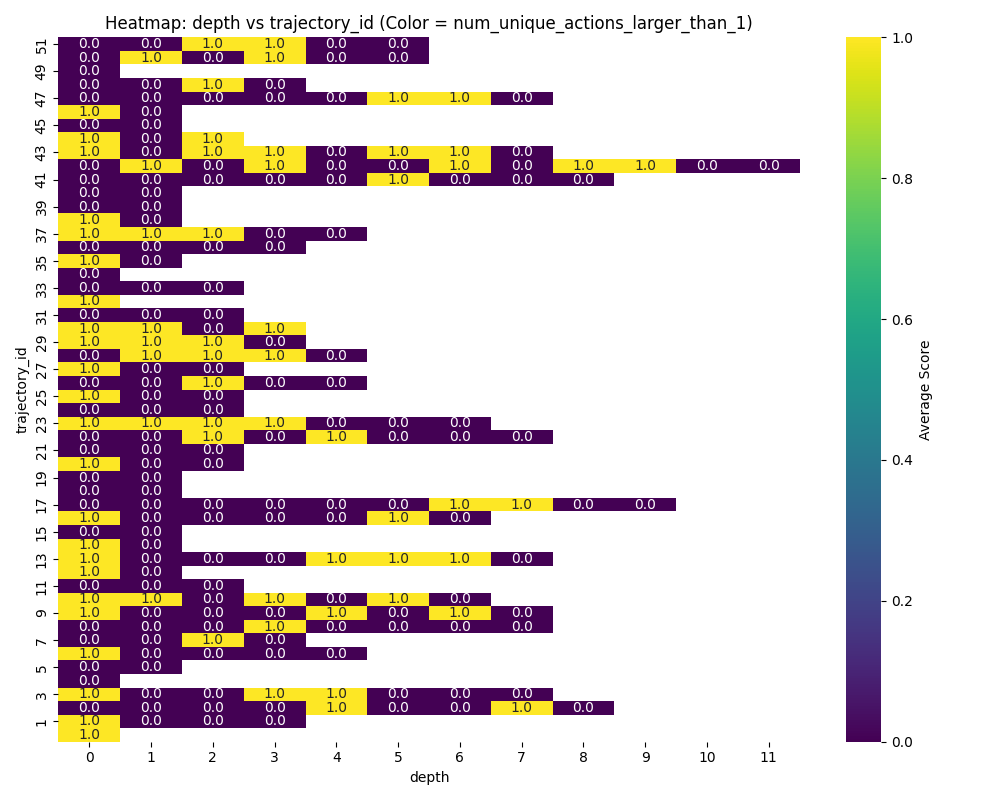
\includegraphics[width=0.95\textwidth]{figures/trajectory_data/num_unique_heatmap.png}
    \caption{Heatmap of turn-level action diversity under resampling.
    Each cell corresponds to a state indexed by (trajectory id, assistant-call depth).
    We sample the model multiple times from the \emph{same} prefix and mark whether more than one unique structured action is produced ($\mathbf{1}[U(s_t)>1]$).
    Yellow ($1$) indicates multiple distinct actions; purple ($0$) indicates a single action across samples.
    Blank cells correspond to depths beyond the trajectory length.
    The sparsity of high-diversity cells supports the premise that only a small subset of turns are true branching points, motivating pivot-focused updates.}
    \label{fig:unique_actions_heatmap}
\end{figure*}

\paragraph{From sparse branching to sparse advantage.}
The diversity statistic in Figure~\ref{fig:unique_actions_heatmap} is not itself an advantage estimate, but it is a useful operational proxy for where the policy’s \emph{structured} action distribution is non-trivial.
In tool-use settings, turns that admit multiple distinct tool/argument actions are typically exactly those where outcomes can diverge sharply (correct tool call versus failure or costly recovery), which is when turn-level advantages tend to be large.
Conversely, when the policy consistently emits a single structured action at a prefix, the next step is often constrained by the transcript and tool outputs, and alternative actions are either equivalent at the task level or clearly unhelpful.
This motivates focusing our formalism and optimization on states where the turn-level action-value landscape is \emph{not} flat.

\begin{definition}[Turn-level advantage gap]
\label{def:gap}
Fix $(c,\pi)$.
Define the \emph{advantage gap} at state $s$ as
\begin{equation}
\label{eq:gap}
\mathrm{Gap}_c^\pi(s)
=
\max_{a\in\mathcal{A}_c(s)}\big(Q_c^\pi(s,a)-V_c^\pi(s)\big)
=
\max_a A_c^\pi(s,a).
\end{equation}
\end{definition}

\begin{definition}[Pivot state]
\label{def:pivot}
A state $s$ is a \emph{pivot} if $\mathrm{Gap}_c^\pi(s)\ge \delta$ for some threshold $\delta>0$, or if it lies among the top-$K$ states by $\mathrm{Gap}_c^\pi$ within a trajectory.
\end{definition}

\paragraph{Why pivots matter.}
At a pivot, there exists a turn action that is substantially better than the baseline, so learning to assign it higher probability can change the episode outcome.
At non-pivots, $Q(s,a)\approx V(s)$ for all plausible $a$, so the policy-gradient contribution is small.

\begin{proposition}[Non-pivot states contribute little to the turn-level gradient]
\label{prop:nonpivot_small}
Assume $\|\nabla_\theta \log \pi_\theta(a\mid s)\|\le G$.
If $|A_c^{\pi_\theta}(s,a)|\le \varepsilon$ for all $a$ at some state $s$, then
\[
\left\|
\E_{a\sim\pi_\theta(\cdot\mid s)}
\big[\nabla_\theta \log \pi_\theta(a\mid s)\,A_c^{\pi_\theta}(s,a)\big]
\right\|
\le
G\varepsilon.
\]
\end{proposition}

\begin{proposition}[Gradient truncation bound (pivot-only updates)]
\label{prop:trunc}
Let $\mathcal{P}$ be a pivot set and assume that for all $s\notin\mathcal{P}$ we have
$\max_a |A(s,a)|\le \varepsilon$.
Then the difference between the full turn-level gradient and the pivot-only gradient is bounded by
\[
\left\|\nabla_\theta J - \E\big[\mathbf{1}[s\in\mathcal{P}]\nabla_\theta\log\pi_\theta(a\mid s)A(s,a)\big]\right\|
\le
G\varepsilon.
\]
\end{proposition}

Proposition~\ref{prop:trunc} is deliberately simple:
if the turn-level advantage is sparse, concentrating updates on pivots introduces limited bias while saving substantial compute.



\section{Estimating turn-level values without dense branching}
\label{sec:qv}

Turn-level RL still requires comparing $Q(s,a)$ across candidate turn actions $a$ at intermediate prefixes $s$.
Dense branching rollouts from many prefixes is expensive for long-horizon tool use.
PivotRL uses a proxy that leverages two readily available components in tool benchmarks: a strong teacher and a verifier.

\paragraph{Teacher + verifier proxy.}
Let $\pi_T$ be a strong teacher and $\mathcal{V}$ an automated verifier that returns $1$ on success and $0$ otherwise.
Generate teacher trajectories and keep only those accepted by $\mathcal{V}$.
For a state $s$ on an accepted teacher trajectory, denote the teacher turn as $a_T(s)$.
PivotRL uses a proxy label
\begin{equation}
\label{eq:proxyQ}
\widetilde Q(s,a) = \mathbf{1}[a=a_T(s)],
\end{equation}
\begin{equation}
\widetilde V^{\pi_\theta}(s)=\E_{a\sim\pi_\theta(\cdot\mid s)}[\widetilde Q(s,a)]=\pi_\theta(a_T(s)\mid s).
\end{equation}
This yields a proxy advantage $\widetilde A(s,a)=\widetilde Q(s,a)-\widetilde V^{\pi_\theta}(s)$.

\paragraph{When is this justified?}
At pivots in tool calling, action values are often close to binary: a narrow set of correct tool calls keeps the episode on a successful path, and most deviations do not recover.
The proxy in~\eqref{eq:proxyQ} is designed for this regime.

\begin{assumption}[Near-binary turn values at pivots]
\label{assump:binary}
At pivot states $s$, there exists a high-value action $a^\star(s)$ such that
$Q(s,a^\star(s))=1$ and $\max_{a\neq a^\star(s)} Q(s,a)\le \varepsilon$ for small $\varepsilon$.
\end{assumption}

\begin{proposition}[Proxy baseline error shrinks as the policy improves]
\label{prop:proxy}
Under Assumption~\ref{assump:binary}, letting $p=\pi_\theta(a^\star(s)\mid s)$,
\[
0 \le V(s)-\widetilde V(s) \le \varepsilon(1-p).
\]
\end{proposition}

\subsection{Bridging SFT with RL}

Supervised Fine-Tuning (SFT) Gradient can be rewritten as Policy Gradient via Importance Sampling~\citep{wu2025generalization}.
\begin{align*}
&~ \nabla_\theta \mathcal{L}_{\text{SFT}}(\theta) = \mathbb{E}_{(s, a^\star) \sim d_{\sft}} \left[ -\nabla_\theta \log \pi_\theta(a^\star \mid s) \right] \\
= &~ \mathbb{E}_{(s,a) \sim d^{\pi_\theta}_c} \frac{d_{\sft}(s,a)\mathbf{1}[a =a^\star]}{d^{\pi_\theta}_c} \left[ -\nabla_\theta \log \pi_\theta(a \mid s) \right] \\
= &~ -\mathbb{E}_{(s,a) \sim d^{\pi_\theta}_c} \left[ {\color{blue}w_{\sft}(s,a)} \nabla_\theta \log \pi_\theta(a \mid s) {\color{blue}r_{\sft}(s, a)} \right].
\end{align*}
with a reward as an indicator function of matching the expert trajectory and an importance weighting
\begin{align*}
w_{\sft}(s,a) = \frac{d_{\sft}(s,a)}{d^{\pi_\theta}_c}, \quad r_{\sft}(s, a) = \mathbf{1}[a =a^\star].
\end{align*}

While SFT reward $r_{\sft}$ achieves strong in-domain performance improvement due to teacher-forcing, its importance weight $w_{\sft}$ induces an distribution shift from the on-policy occupancy measure, leaning to poor generalizability.
To achieve the best of both worlds of SFT and RL, \name uses the same reward objective with a different pivot-based, value-sensitive weights:
\begin{align*}
w_{\name}(s,a) =\mathbf{1}(\mathrm{Gap}_c^\pi(s) > \delta)/Z
\end{align*}
where $Z = \E_{(s,a) \sim d^{\pi_\theta}_c}[\mathbf{1}(\mathrm{Gap}_c^\pi(s) > \delta)]$ is a normalization constant.
This gives rise to the following policy gradient that bridges SFT with RL
\begin{align*}
&~ \nabla_\theta \mathcal{L}_{\text{\name{}}}(\theta) = \\
&~ -\mathbb{E}_{(s,a) \sim d^{\pi_\theta}_c} \left[ {\color{blue}w_{\name}(s,a)} \nabla_\theta \log \pi_\theta(a \mid s) {\color{blue}r_{\sft}(s, a)} \right].
\end{align*}


